\chapter{Behind the Scenes}

The tutorial walked through a number of examples that illustrate the
structure of code written for LLAMAComm.  This chapter fills in some
of the details concerning how LLAMAComm works in the background.  We
will look at how the simulation is moderated by the arbitrator and
the signal processing involved in combining signals from multiple
sources.  These details are pertinent for developing more advanced
simulations and understanding the results.

\section{Simulation Execution}\label{sec:simExecution}

The main program loop of LLAMAComm is shown in Figure
\ref{fig:mainLoop}. This loop represents the core of the simulator.
There are two primary blocks: \verb+Run Controllers+ and
\verb+Run Arbitrator+. The first calls the node controller functions, while
the second controls the simulation's execution order and calls the
module transmit and receive functions.  It is this second
block---the arbitrator---that is truly responsible for coordinating
the execution of the simulation.

\begin{figure}[h]
\centering
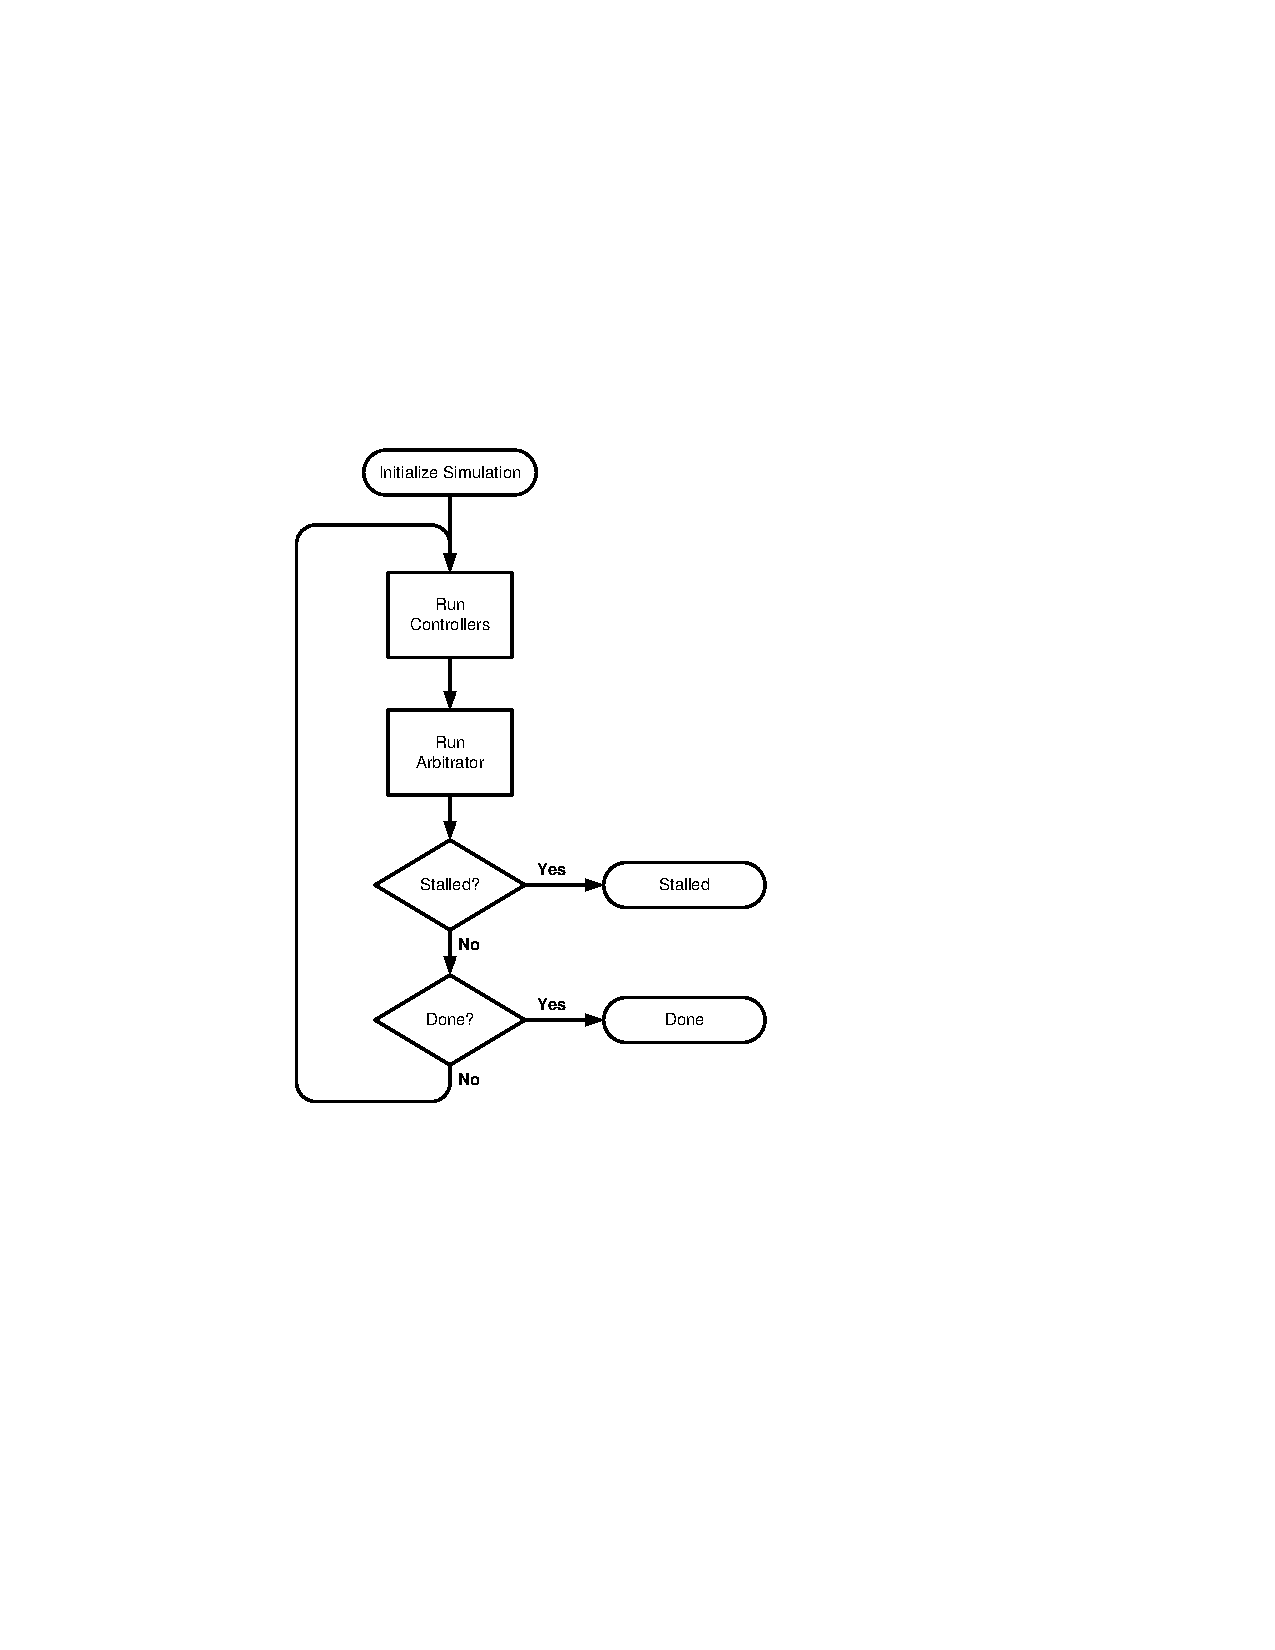
\includegraphics[height=4in]{figs/Main_Loop_Flowchart}
\caption{Flowchart of LLAMAComm's main program loop}
\label{fig:mainLoop}
\end{figure}

\subsection{Run Controllers}

In the \verb+Run Controllers+ block, the controller function in each
node is executed once.  For digital designers, this is analogous to
providing one clock edge to a finite state machine implemented in
digital logic.  The state is stored within the node object.  When
the controller function is \emph{clocked}, it is given the
opportunity to analyze its inputs, set some outputs, and change its
state. Controller functions should be written so that the order in
which they are called relative to other controllers should not
matter. The tutorial in Chapter~\ref{chp:tutorial} covered the
implementation of controller functions in great detail.

\subsection{Run Arbitrator} \label{sec:runArbitrator}

In the \verb+Run Arbitrator+ block, the arbitrator looks at all the
nodes in the scenario, and satisfies as many outstanding requests as
possible.  A simplified version of the arbitrator's flowchart is
shown in Figure \ref{fig:arbitFlowchart}.  The arbitrator sees only
the modules in a scenario.  In fact, it only looks at the module
properties dealing with requests to transmit and receive.

\begin{figure}[!h]
\centering
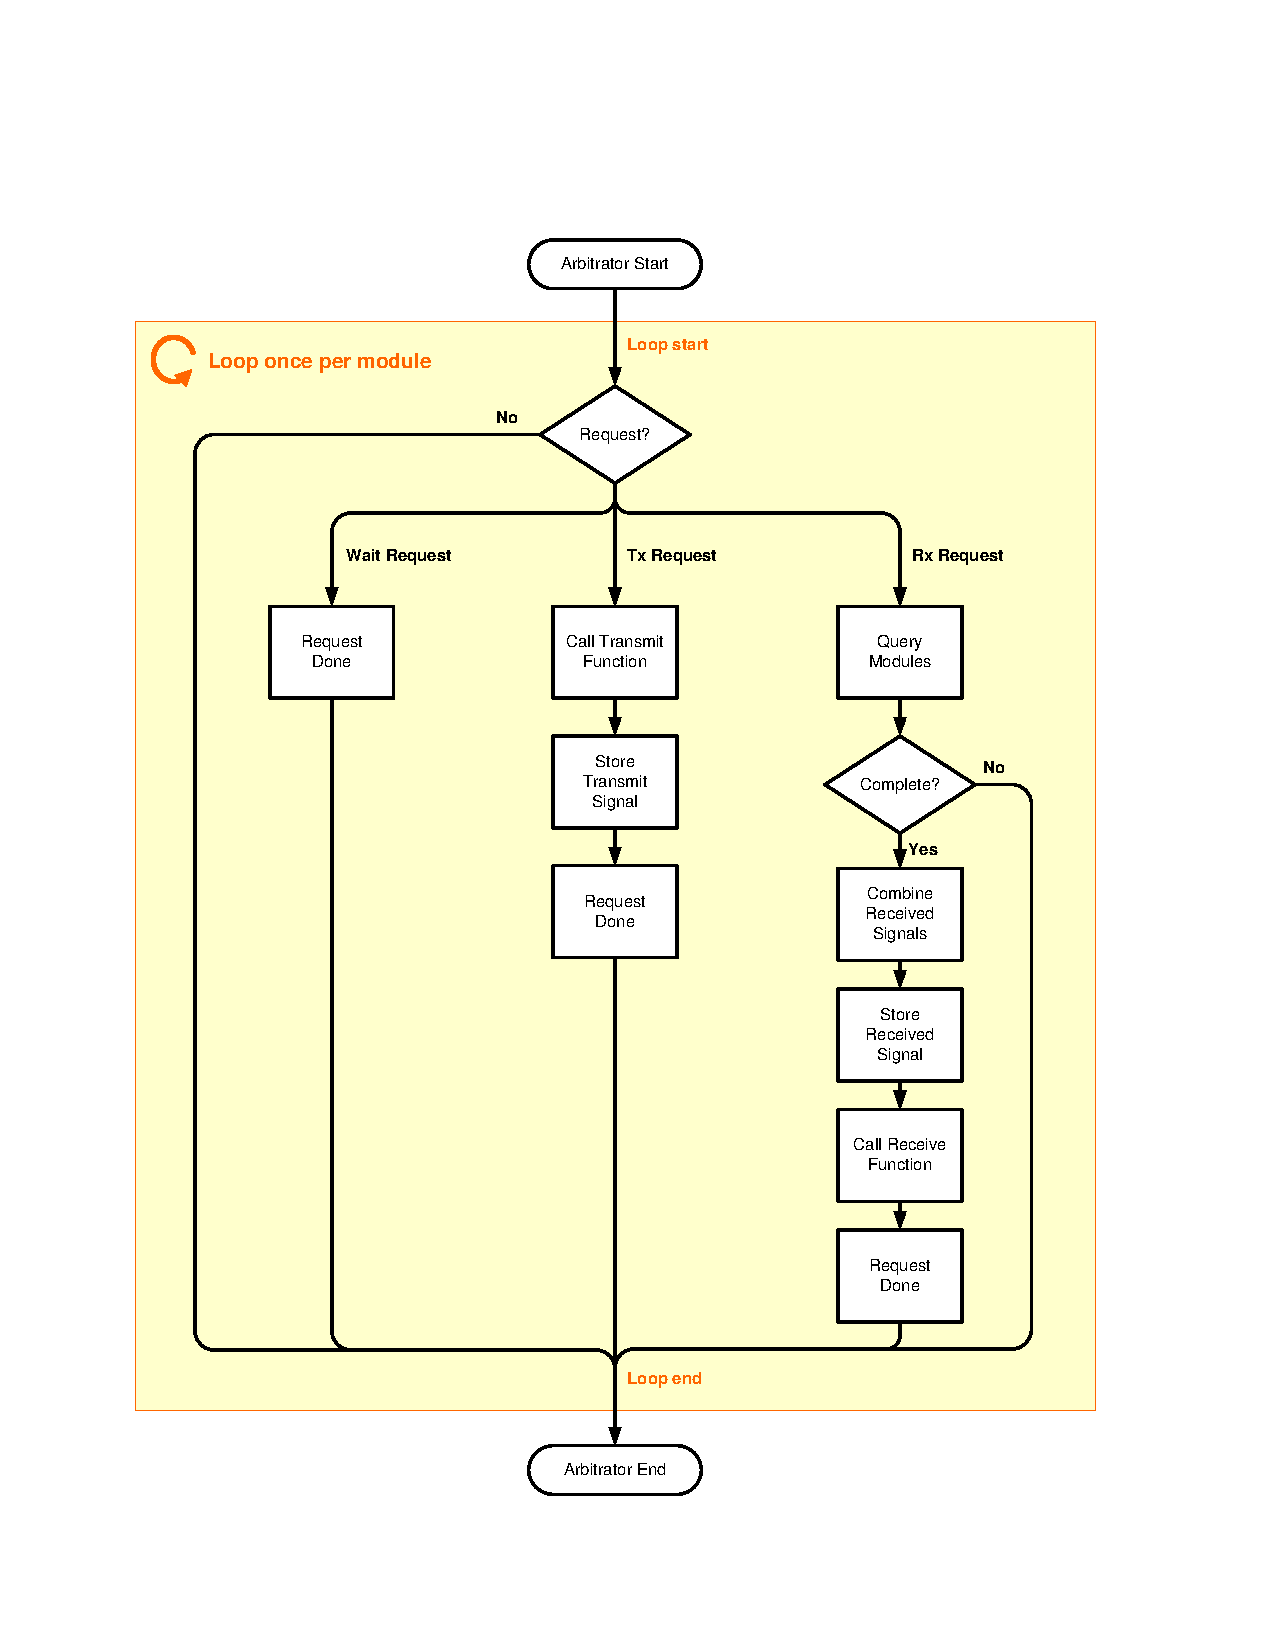
\includegraphics[height=6in]{figs/Arbitrator_Flowchart}
\caption{Flowchart of the arbitrator}
\label{fig:arbitFlowchart}
\end{figure}

The arbitrator flowchart (Figure \ref{fig:arbitFlowchart}) contains
a block labeled \verb+Query Modules+ that requires special
attention. What this block does is ask every other module in the
scenario, ``Do you have transmit data for samples x to y?'' Modules
can respond with one of three messages: \emph{data available},
\emph{not transmitting in-band}, or \emph{not ready}. \emph{Data
available} means that the transmit data has been calculated and is
ready to go. \emph{Not transmitting in-band} means that either the
module is not a transmitter (never transmits), or is transmitting
out of band during the requested segment. \emph{Not ready} means
that the module has not yet calculated the data for that segment and
cannot reply with certainty.  A query is considered complete if no
module responds \emph{not ready}.  This mechanism ensures that a
receiver does not attempt to receive a segment of data until all
transmitters in the requested time period have already transmitted.

This is also a good time to note that changing the center frequency
of a module is allowed on a segment-by-segment basis.  As a result,
the arbitrator must also check for frequency overlap in each segment
when querying the modules.

\subsection{Stepping Through an Example Scenario}

A good way to understand the interaction between the controllers and
the arbitrator is by studying an example from the perspective of the
arbitrator. Figures \ref{fig:arbitEx1} to \ref{fig:arbitEx3}
illustrate this process by stepping through a very short scenario.


\begin{figure}[!h]
\centering \mbox{
    \subfigure[Loop 1: Start]{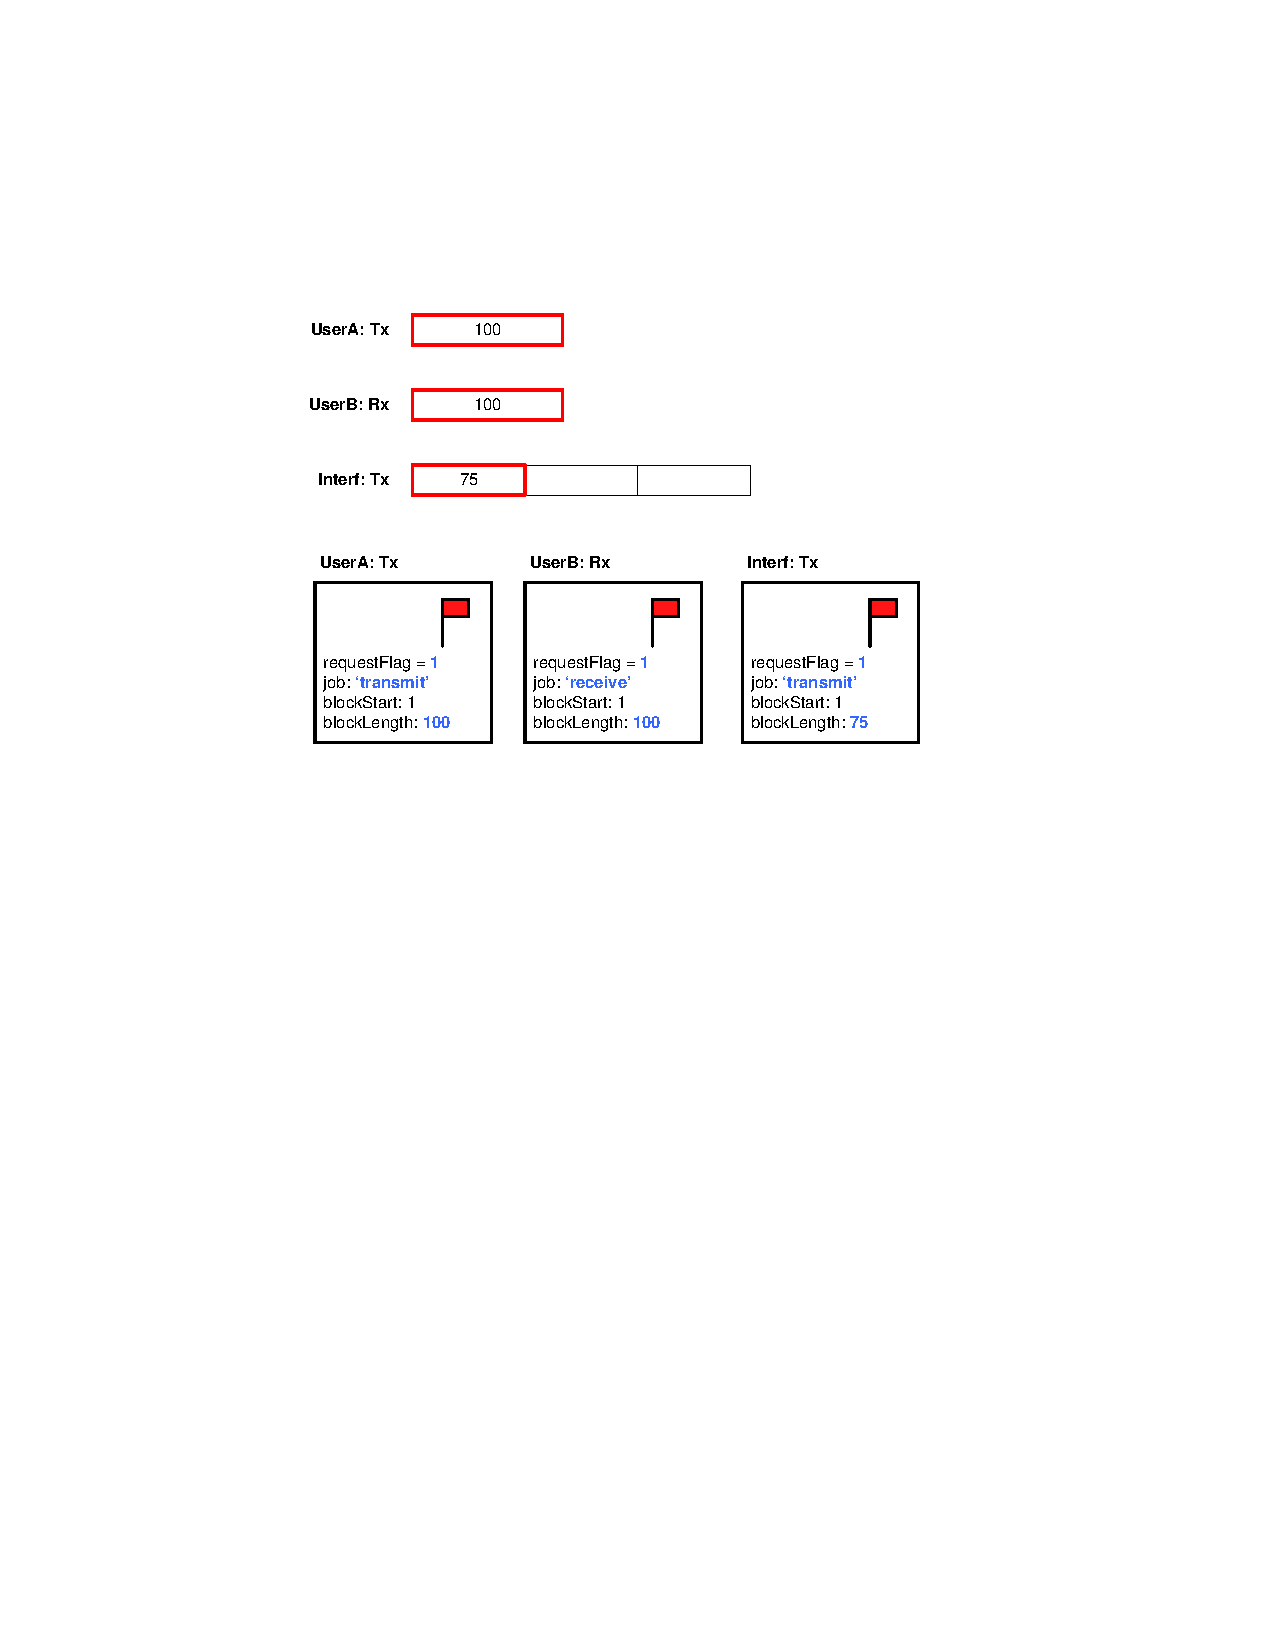
\includegraphics[width=3in]{figs/Arbitrator_Ex_1}} \quad
    \subfigure[Loop 1: End]{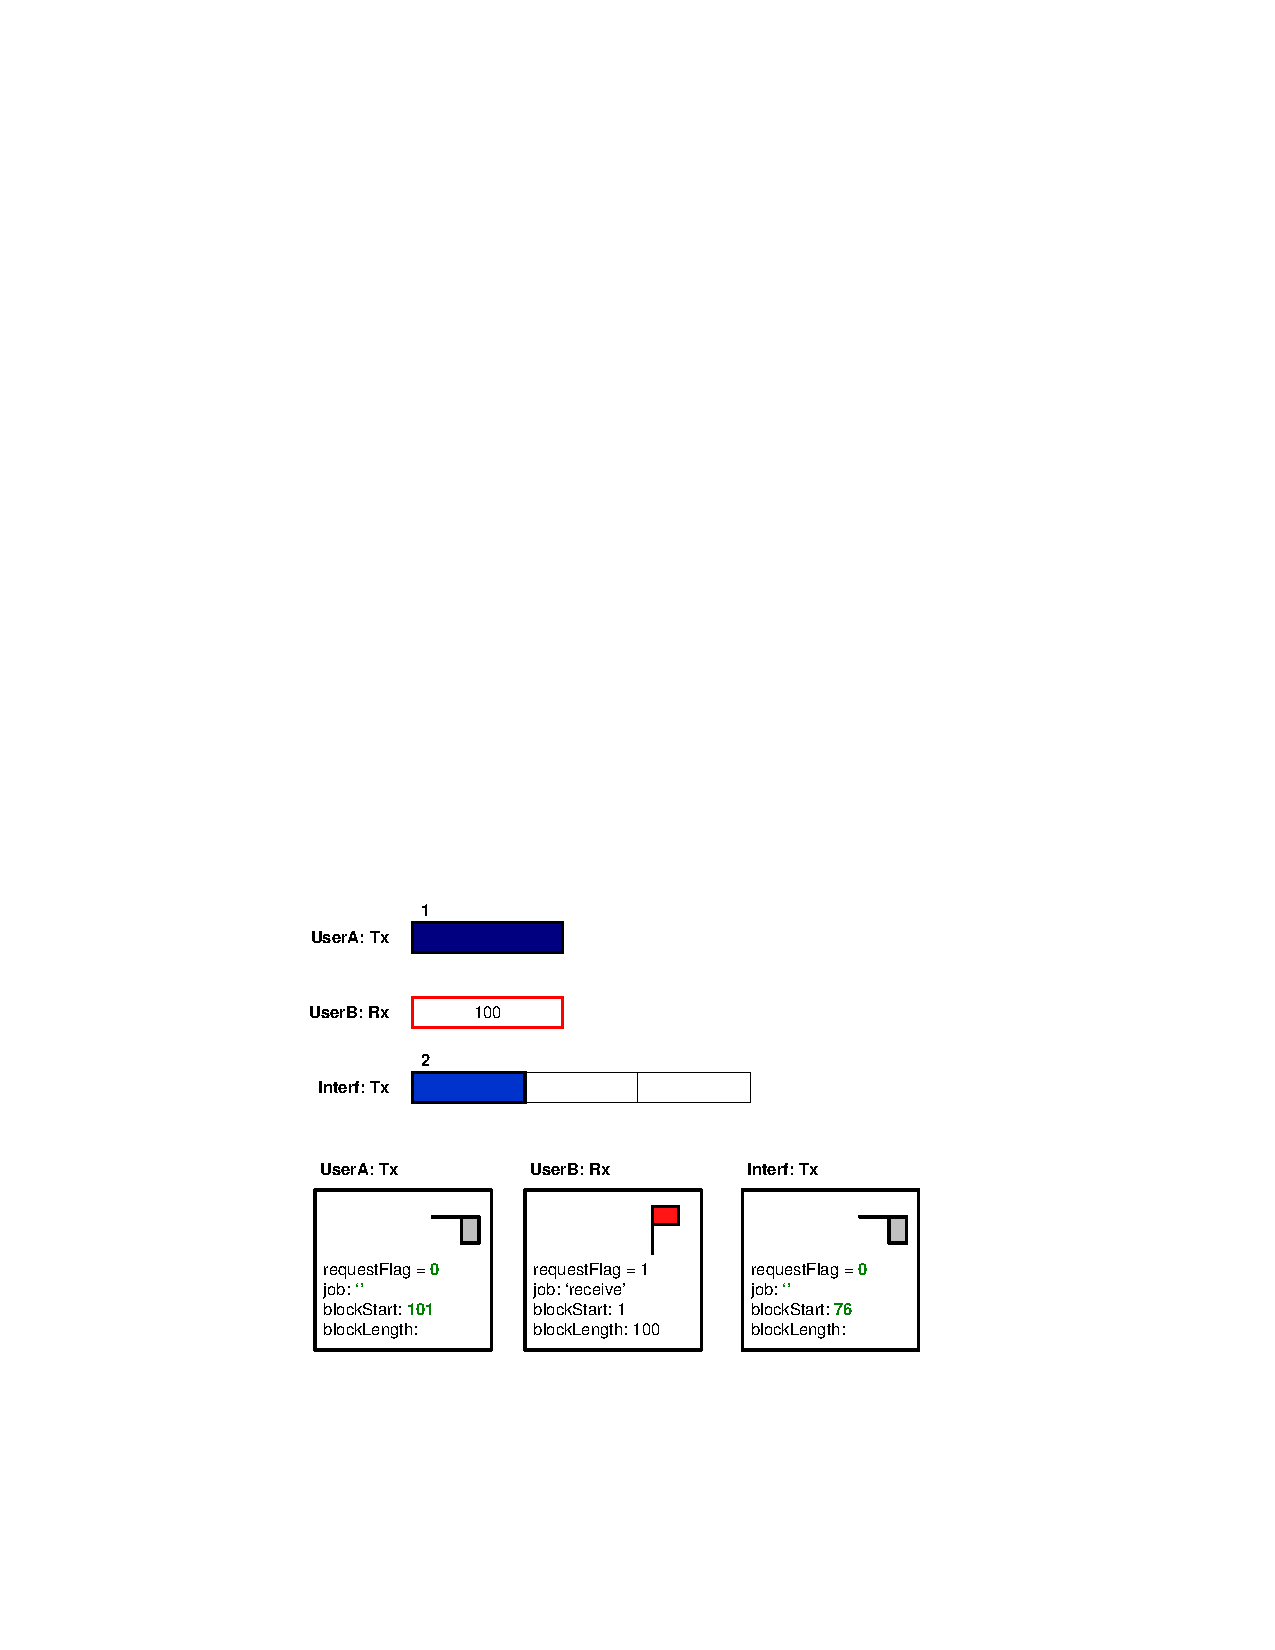
\includegraphics[width=3in]{figs/Arbitrator_Ex_1a}}
} \caption[Arbitrator Example: Loop 1]{Example simulation at the
start and end of the first pass of \tt{RunArbitrator()}}
\label{fig:arbitEx1}
\end{figure}

Figure \ref{fig:arbitEx1} shows an example of the arbitrator's view
of the simulation before and after the first pass of
\verb+RunArbitrator()+.  This example consists of three modules:
\verb+UserA:Tx+, \verb+UserB:Rx+, and \verb+Interf:Tx+.  These
modules are represented as boxes containing a request flag.  The
properties shown in each box are the module properties relevant to a
request.  The two user modules have controller functions that are
written to transmit and receive a single 100-sample segment of
signal.  The interference module is configured to transmit three,
75-sample segments.

In Figure \ref{fig:arbitEx1}(a), the controller functions have set
the properties shown in blue.  The timing diagram above the picture
of the modules, shows the progress of the simulation so far.  At the
start, all modules have an outstanding request to the arbitrator.
The arbitrator attempts to process each of these modules in turn.
The steps are listed below as a mock transcript of the arbitrator
execution.

\begin{verbatim}
        Process UserA:Tx
            Request outstanding
            Call transmit function
            Save transmit waveform to disk
            Request done
        Process UserB:Rx
            Request outstanding
            Query results = not complete
            Skipping request
        Process Interf:Tx
            Request outstanding
            Call transmit function
            Save transmit waveform to disk
            Request done
\end{verbatim}

The arbitrator is operating left to right in this example. First,
the request to transmit by \verb+UserA:Tx+ is processed. After
calling the transmit function and writing the resulting baseband
data to disk, the arbitrator lowers the request flag, deletes the
outstanding job name, and increments the start index for the next
block.  The request to receive by \verb+UserB:Rx+ is then skipped
because the required data is not yet available. \verb+UserB:Rx+
needs data from sample 1 to 100.  During the first pass
\verb+UserA:Tx+ has data ready, but \verb+Interf:Tx+ responds
\emph{not ready} to the query. After \verb+UserB:Rx+ is skipped, the
request from \verb+Interf:Tx+ is satisfied.

\begin{figure}[!h]
\centering \mbox{
    \subfigure[Loop 2: Start]{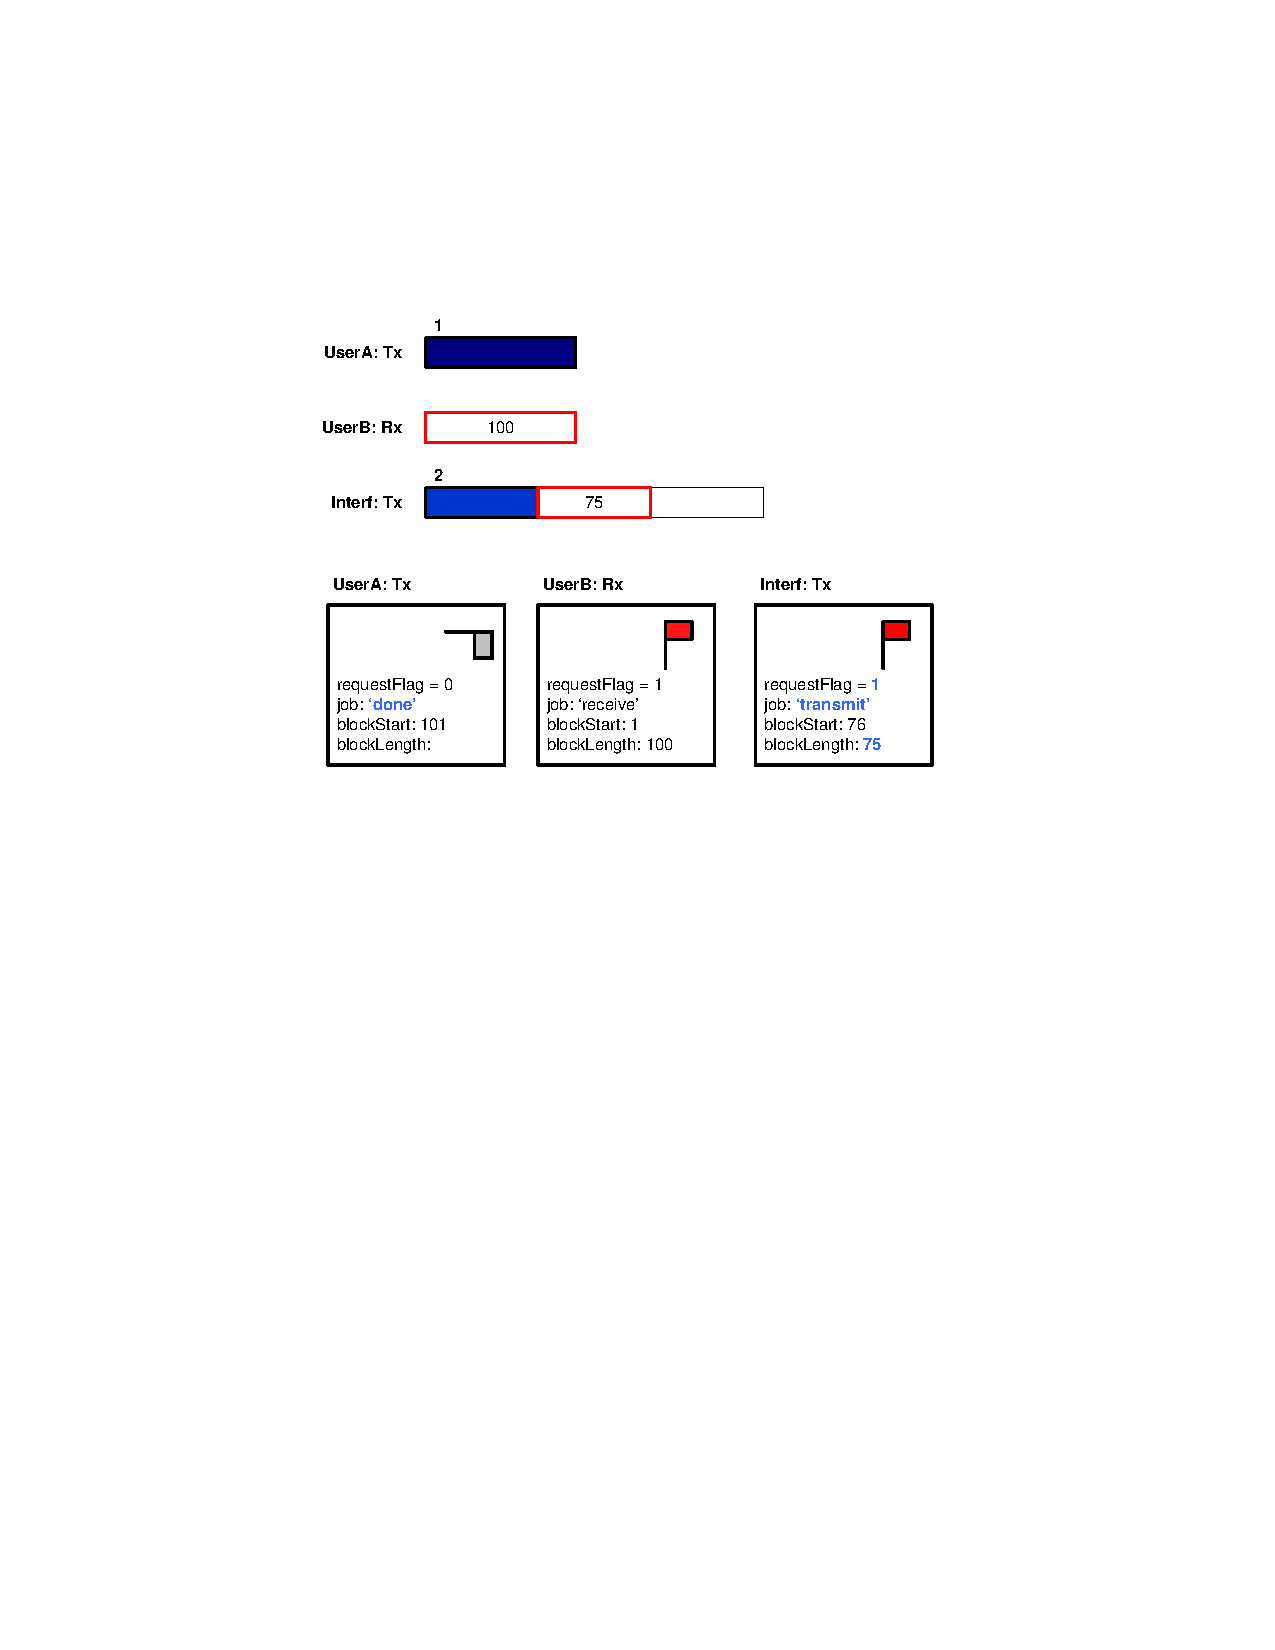
\includegraphics[width=3in]{figs/Arbitrator_Ex_2}} \quad
    \subfigure[Loop 2: End]{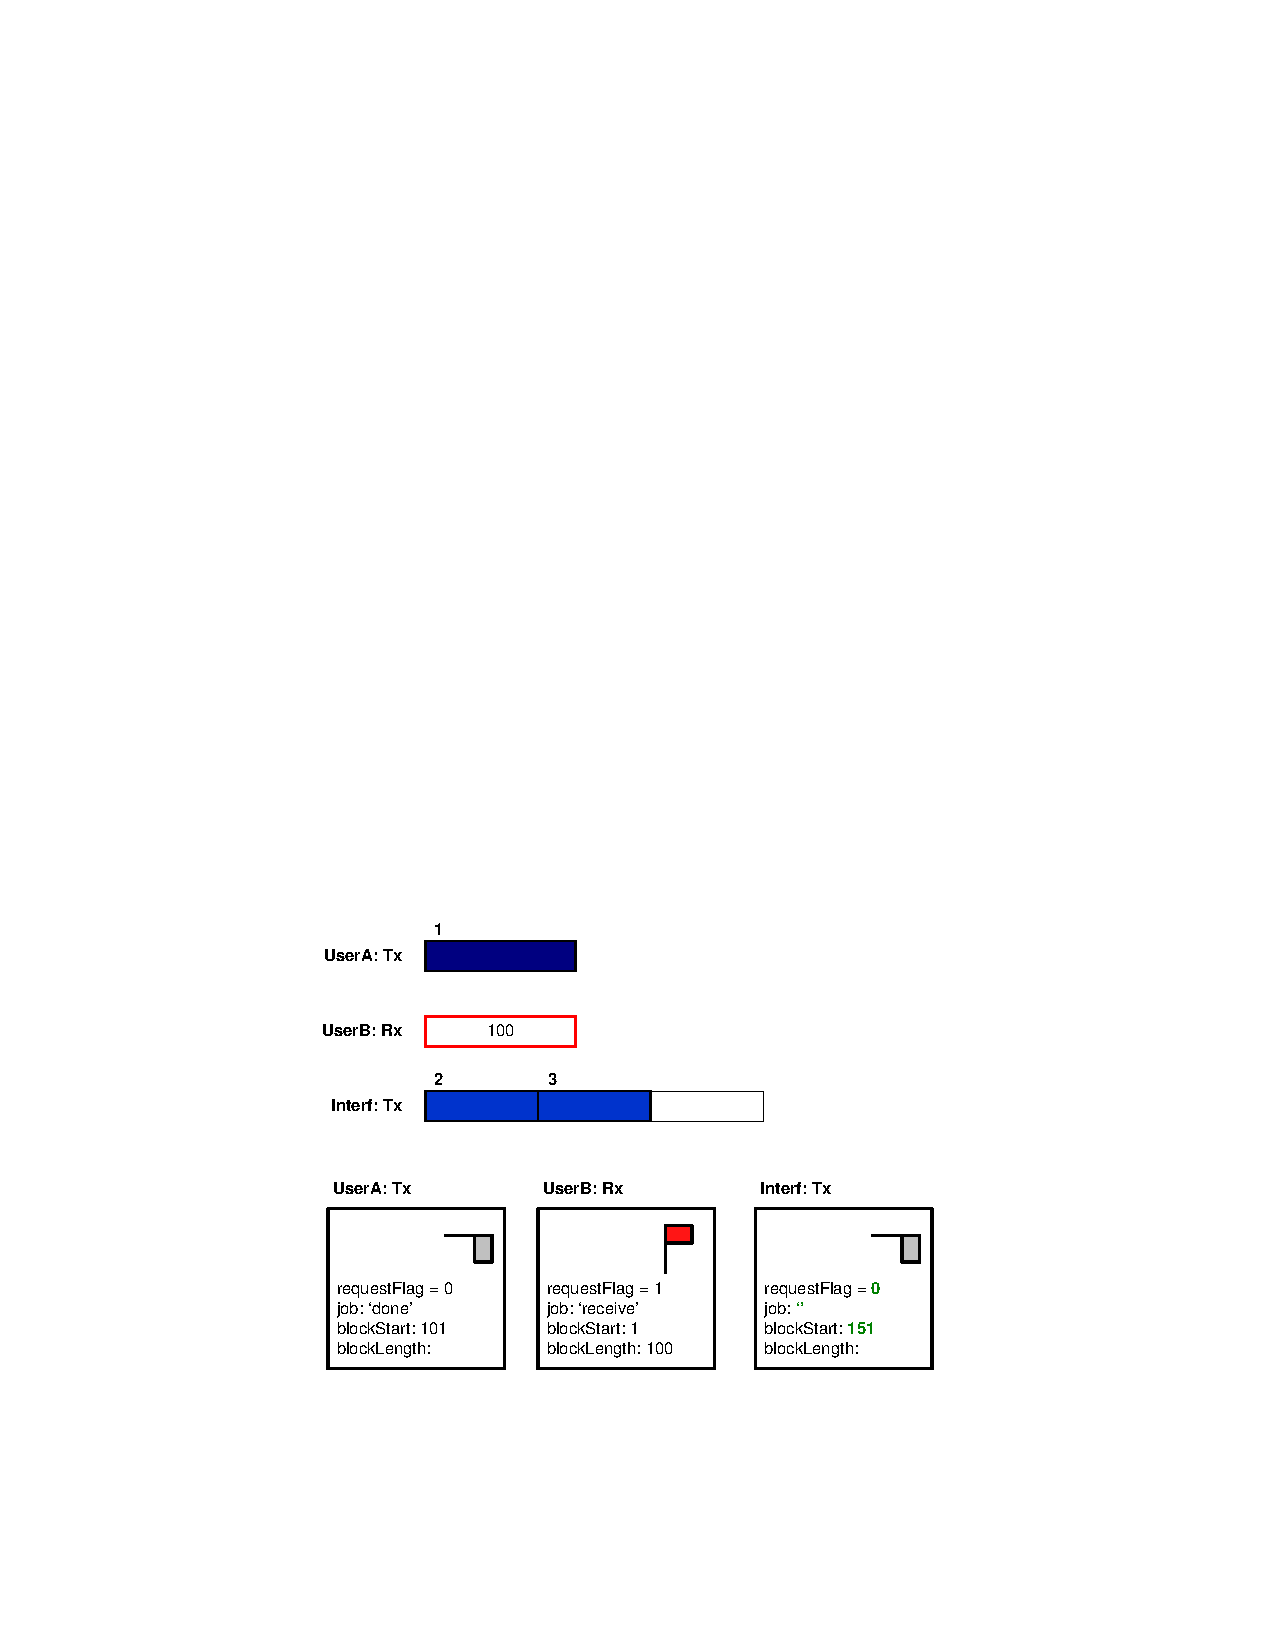
\includegraphics[width=3in]{figs/Arbitrator_Ex_2a}}
} \caption[Arbitrator Example: Loop 2]{Example simulation at the
start and end of the second pass of \tt{RunArbitrator()}}
\label{fig:arbitEx2}
\end{figure}

Figure \ref{fig:arbitEx2} shows the example at the beginning and end
of the second pass of the arbitrator.  \verb+UserA:Tx+'s controller
has tagged the module as ``done'', so from now on, \verb+UserA:Tx+
will be ignored by the arbitrator.  The request from \verb+UserB:Rx+
is still outstanding and has not changed.  The controller function
for the interference module has issued another transmit request. The
mock transcript for this iteration of the arbitrator follows.

\begin{verbatim}
        Process UserA:Tx
            Skip (module marked as Done)
        Process UserB:Rx
            Request outstanding
            Query results = not complete
            Skipping request
        Process Interf:Tx
            Request outstanding
            Call transmit function
            Save transmit waveform to disk
            Request done
\end{verbatim}

In this pass, \verb+UserB:Rx+ is again skipped because
\verb+Interf:Tx+ has not yet transmitted and therefore responds
\emph{not ready}.  \verb+Interf:Tx+ is able to transmit at the end
of the iteration, and its waveform is saved to disk.

\begin{figure}[!h]
\centering \mbox{
    \subfigure[Loop 3: Start]{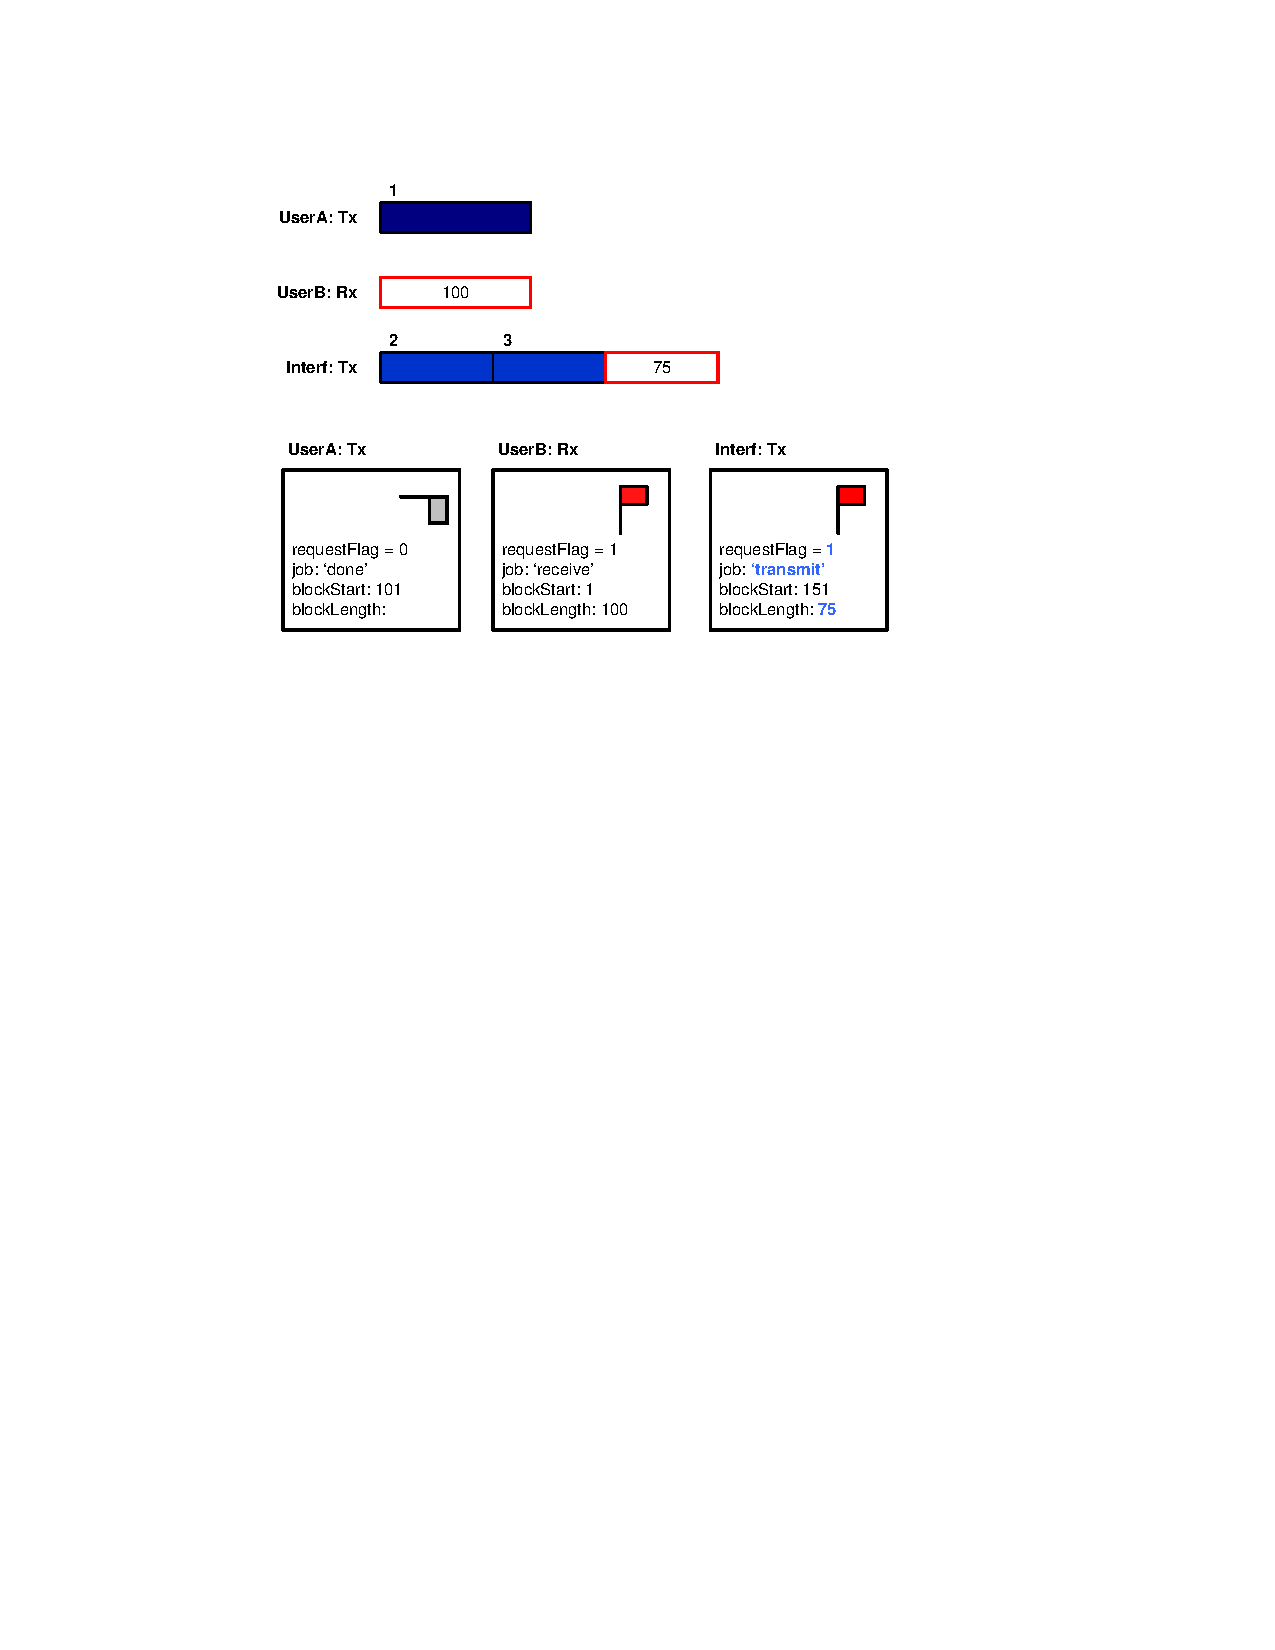
\includegraphics[width=3in]{figs/Arbitrator_Ex_3}} \quad
    \subfigure[Loop 3: End]{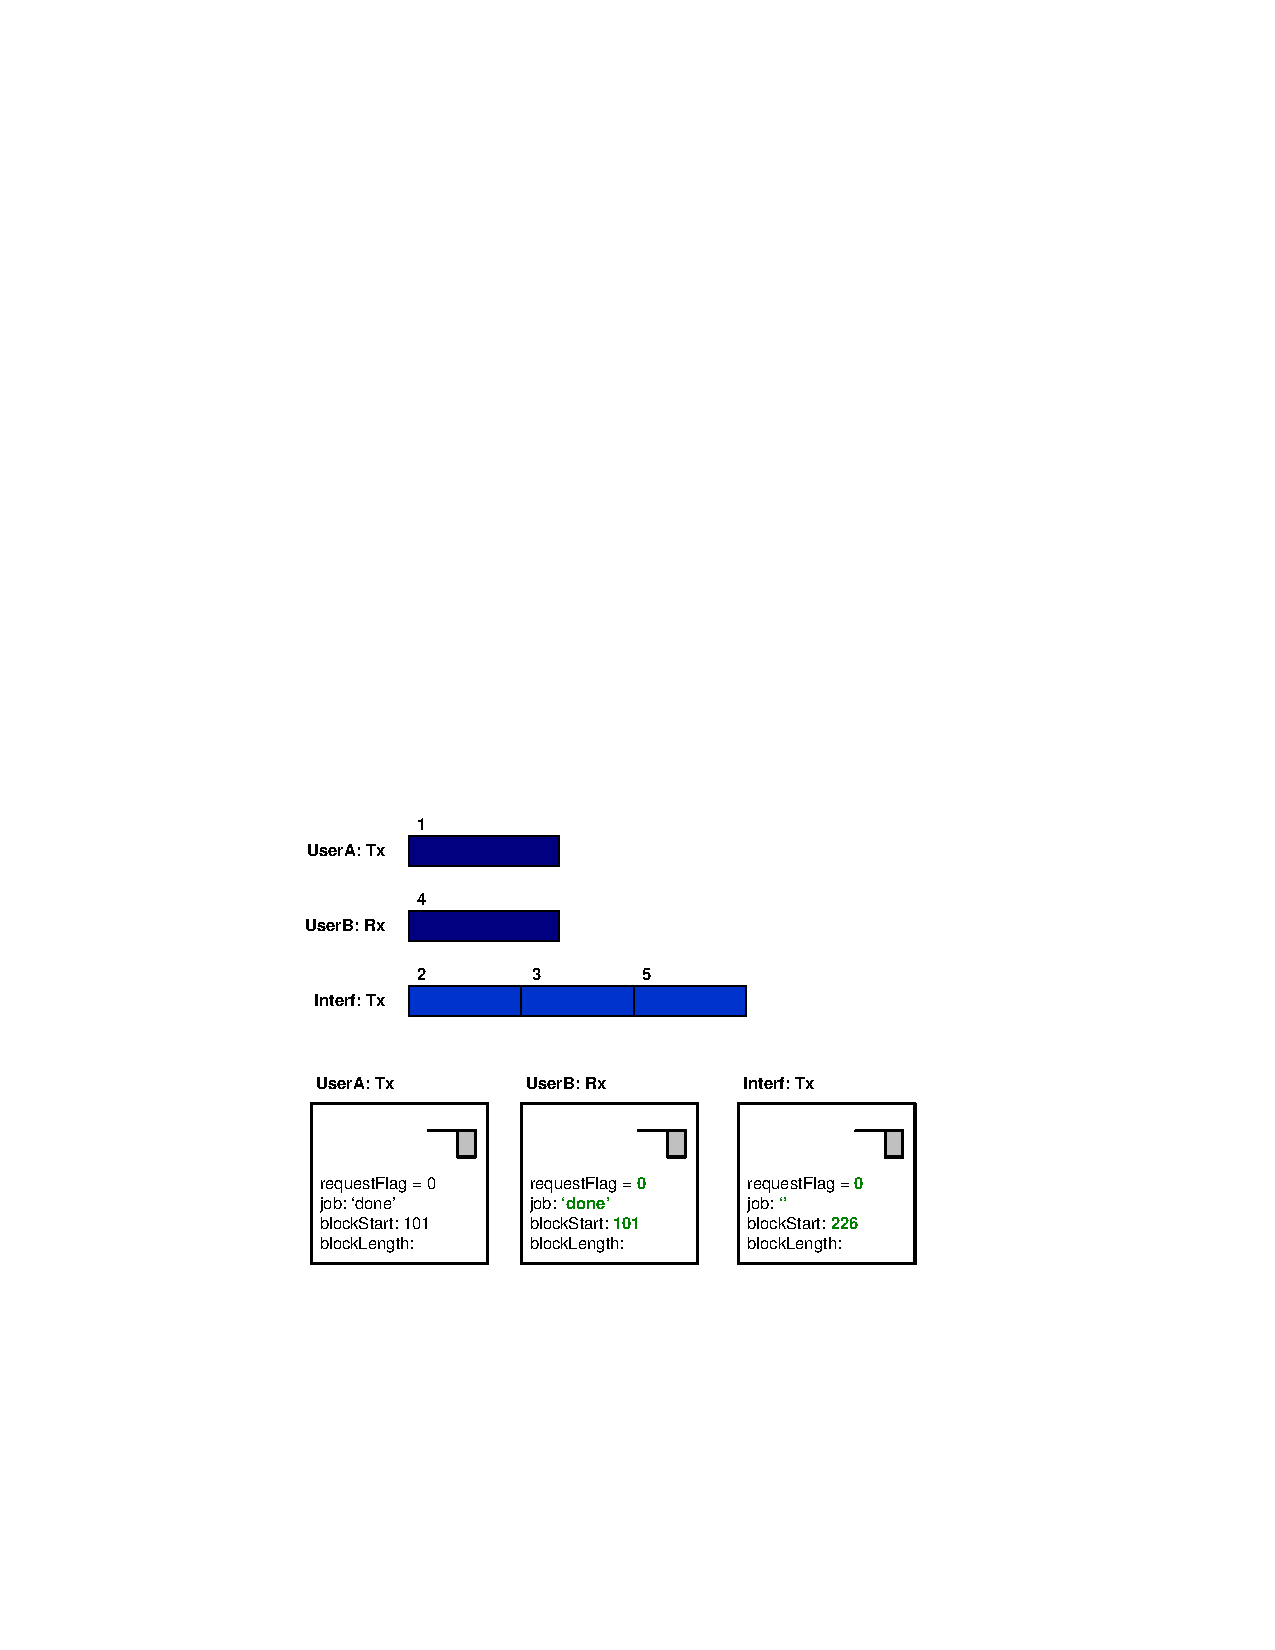
\includegraphics[width=3in]{figs/Arbitrator_Ex_3a}}
} \caption[Arbitrator Example: Loop 3]{Example simulation at the
start and end of the third pass of \tt{RunArbitrator()}}
\label{fig:arbitEx3}
\end{figure}

Figure \ref{fig:arbitEx3} shows the third and final pass of the
arbitrator.  At the start of the iteration, the request from
\verb+UserB:Rx+ is still outstanding.  The interference controller
has requested to transmit another segment.  The transcript follows.

\begin{verbatim}
        Process UserA:Tx
            Skip (module marked as Done)
        Process UserB:Rx
            Request outstanding
            Query results = complete
            Combining received signals
            Save received waveform to disk
            Request done
        Process Interf:Tx
            Request outstanding
            Call transmit function
            Save transmit waveform to disk
            Request done
\end{verbatim}

In this pass, \verb+UserB:Rx+ can finally receive.  The queries to
\verb+UserA:Tx+ and \verb+Interf:Tx+ both respond \emph{data ready} since data
for samples 1 to 100 are available in all transmit modules.  The relevant
portions of data are loaded from disk and combined as described in Section
\ref{sec:combineSignal}.  Signal combining adds the contributions from all
segments that overlap the requested receive segment in time and frequency.  The
multichannel propagation models are called from within the signal combining
block to generate the simulated baseband received signal.  This baseband signal
is passed into the user-defined receive function and demodulated.  The receive
request for \verb+UserB:Rx+ is marked as complete.  Following this, the
interference module request is satisfied as usual.

From the previous example, it is easy to see that requests to transmit are
never stalled.  It is only receive requests that force the simulation to
execute out of order.

The operation of the genie channels was not mentioned in this
example.  In practice, genie module requests work much like transmit
requests. Genie transmit requests are processed on the very first
pass. Genie receive module will have to wait no more than one
iteration if the transmitter and receiver are synchronized properly.

\subsection{Ending the Simulation Gently}

Other than crashing or forcibly quitting MATLAB, there are two ways
a simulation may end: all the controller functions must reach a done
state, or the arbitrator decides that the simulation has stalled.

The arbitrator decides that \emph{the simulation has stalled if for
any single iteration of the main program loop there are outstanding
requests, and none could be satisfied}.  This may occur, for
example, if a receive block requires data samples 10000-12000, but
these samples are never available because all the other radios in
the simulation stopped transmitting after 5000 samples.

It is for this reason that modules can be marked as \emph{done}.
This is accomplished by calling \verb+SetModuleRequest()+ with the
\verb+job+ argument set to \verb+`done'+.  Modules marked as
\emph{done} are assumed to be not transmitting for all samples
beyond what is contained in its history. So, in the example
mentioned above, the receive module requesting samples 10000-12000
would proceed by receiving samples with zero signal.

Marking the module as \emph{done} should not be confused with the
controller function's \verb+done+ state. Controller functions are
responsible for returning a status message to the main program loop
that is either \verb+`running'+ or \verb+`done'+.  All controllers
begin by returning \verb+`running'+.  When a controller reaches the
\verb+done+ or \verb+finish+ state, it returns \verb+`done'+ for the
status. When all controllers return \verb+`done'+ for the status,
the main program loop knows that the simulation has successfully
finished.

The half-duplex, full-duplex, and LL MIMO controllers in the example
section (\S\ref{sec:exampleSection}) are careful to mark modules
\emph{done} when finished.  The interference source controllers, in
contrast, reach the \verb+done+ state but do not mark the modules as
\emph{done}. This is so that LLAMAComm will stall if not enough
interference samples are produced.  (We did not want the example
radios to accidentally operate without interference.)

\section{Environment Modeling and Signal Processing}

The environment modeling and signal processing are explained in the following
subsections.

\subsection{Creating Link Objects} The \link\ object is created by the function
\verb+/@envirnoment/BuildLink.m+, which uses sophisticated environment modeling
to build the channel parameters used by the signal processing engine.  For
debugging purposes, the \link\ object also contains the path-loss, the
shadow-loss, and other channel properties (see \secref{linkparams}).%
% Much of
%the code for creating the \link\ was taken verbatim from LLAMAComm's
%predecessor---Cogcom. 
Each \link\ is created as needed. For example, if a
transmit module and receive module have non-overlapping bands, then no \link\
is created between them.

It may occur that the transmit and receive \module\ are contained within the
same node. In the current version of LLAMAComm, a dummy \link\ is created such
that there is no self-interference. Future versions of LLAMAComm will address
the issue of self-interference.

\subsection{Combining Signals}\label{sec:combineSignal}

%
\begin{figure}[!h]
\centering
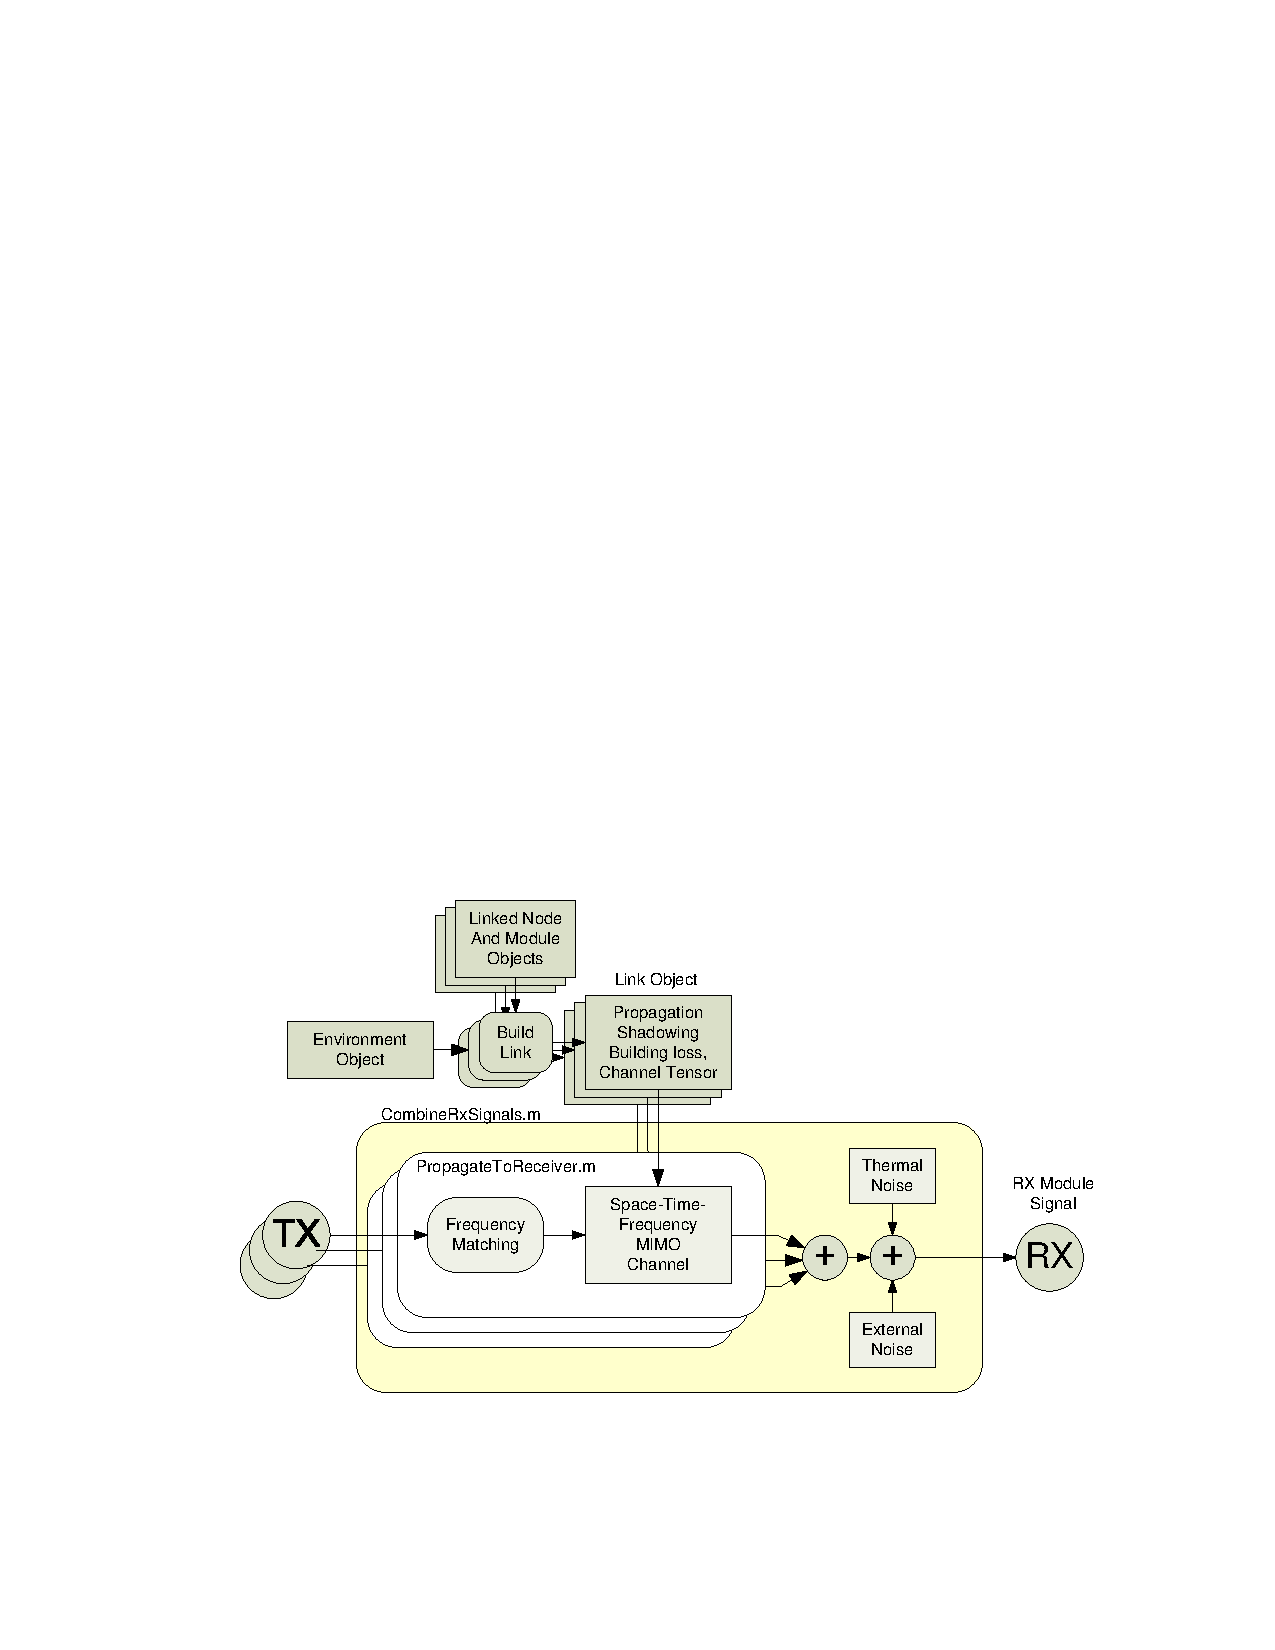
\includegraphics[width=6in]{figs/Combine_Rx}
\caption{Signal processing overview.} \label{fig:combinerx}
\end{figure}
%
%
\begin{figure}[!h]
\centering
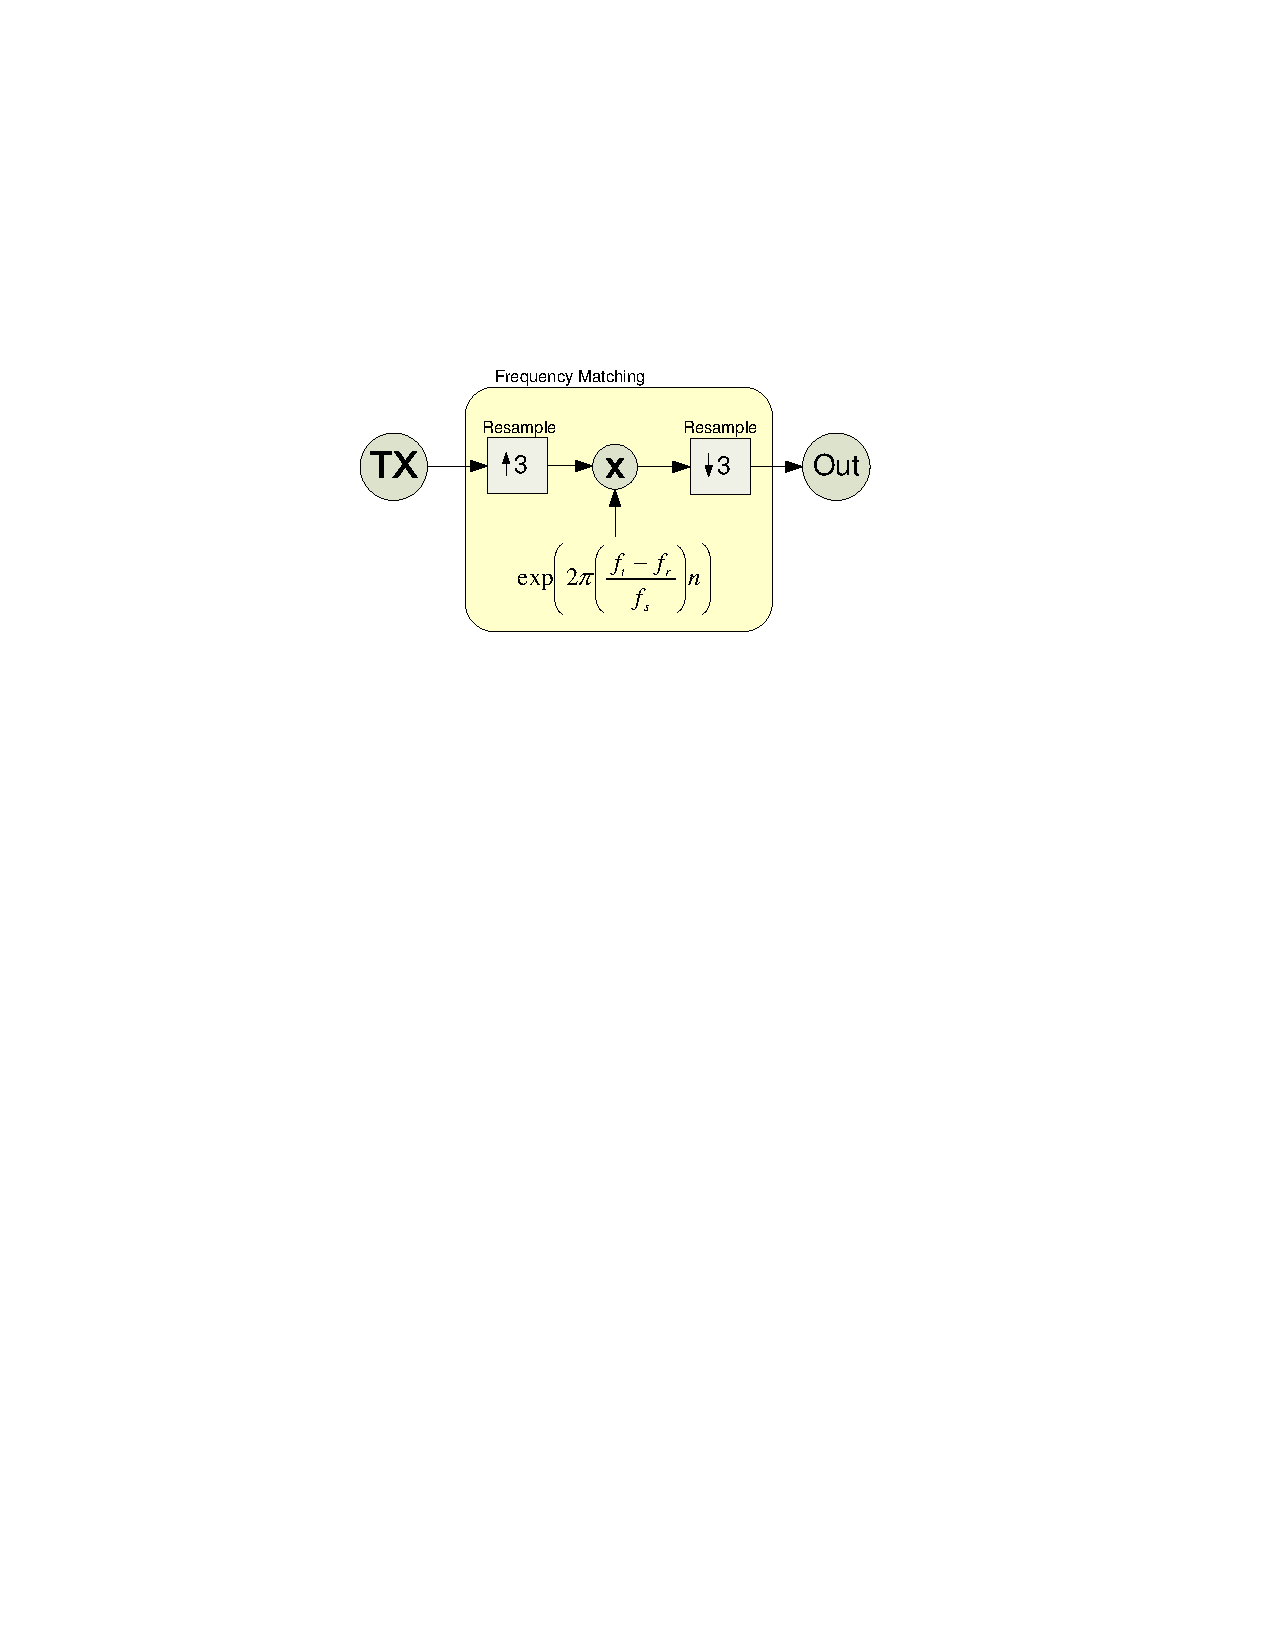
\includegraphics[height=2in]{figs/Freq_Match}
\caption{Frequency matching block diagram.} \label{fig:freqmatch}
\end{figure}
%
The signal processing chassis of LLAMAComm, called by
\verb+@node/RunArbitrator.m+, is the function
\verb+@node/CombineRxSignals.m+.  A block diagram overview of the
signal processing is shown in \figref{combinerx}.
\verb+CombineRxSignals.m+ takes as input the analog signals produced
by the relevant transmit modules, runs these signals through their
respective channels, combines the outputs, and adds white Gaussian
noise. The relevant modules are those whose transmit band overlap
with the band of the receive module.

A chassis needs an engine to operate, and in the case of LLAMAComm,
the signal processing engine is the function
\verb+@link/PropagateToReceiver.m+.  This function reads the
specified transmit waveform from file, applies frequency matching and propagation delays when needed, and finally applies the appropriate physical layer channel
model specified in the pertinent \link\ object.  The result is the
noiseless received signal seen at the receive \module channel
output.

Frequency matching is needed when the transmit and receive modules have
different center frequencies. \Figref{freqmatch} shows the frequency-matching
block diagram. The interpolation and decimation is done on a block-by-block
basis using the MATLAB built-in function \verb+resample.m+.  The function
\verb+resample.m+ assumes the signal is zero outside given the window of
samples; hence, the edges will be mangled.  This can be avoided by setting all
the transmit and receive modules in the same band to the same center frequency,
thereby eliminating the need for frequency matching.  In the future, LLAMAComm
will have the option to perform non-causal processing to eliminate the edge
mangling.

As an example of a case where frequency-matching is necessary, suppose the
simulation sample rate is $f_s = 12.5$ MHz and suppose we have transmit and
receive modules with center frequencies of $f_t = 98$ MHz and $f_r = 100$ MHz,
respectively. The band occupied by the transmit module is $[91.75, 104.25]$
MHz, while the band observed by the receive module is $[93.75, 106.25]$ MHz.
The receiver ``sees'' only the following portion of the transmit signal:
$[93.75, 104.25]$ MHz. We can create the proper received signal by
interpolating, appropriately modulating, and decimating the transmit signal.

\subsection{Local Oscillator Errors} \label{sec:localoscillatorerrors}
This section discusses how LLAMAComm simulates fine local oscillator errors (as opposed to the coarse center frequency mismatches discussed in the previous section).  Each module has two properties regarding the local oscillator: \verb+.loError+ and \verb+.loCorrection+.  Both of these module properties are given in units of parts.  For example, to simulate a local oscillator error of 0.95 parts per million, let \verb+loError = 0.95e-6+, resulting in a frequency offset of, e.g., 950 Hz at a center frequency of 1 GHz.  The \verb+.loError+ module property can only be modified during node construction at the beginning of the simulation.

During simulation, the user can adjust the local oscillator through the \verb+loCorrection+ module property by calling the node method \verb+SetLoCorrection.m+.  For example, to correct the previous local oscillator error of 0.95 parts per million, set \verb+loCorrection = -0.95e-6+.

The fine frequency offset of the link will be calculated relative to the receiver local oscillator error and the receiver center frequency.  For example, given a nominal receive center frequency of \verb+fr+ Hz, the link frequency offset will be: \verb|freqOffset = (loErrorTx + loCorrectionTx - loErrorRx - loCorrectionRx)*fr; % (Hz)|.

The fine frequency offset is the last processing applied to the received signal in \verb+/simulation/@link/PropagateToReceiver.m+ as follows:
\begin{verbatim}
freqOffset = (mTx.loError + mTx.loCorrection ...
            - mRx.loError - mRx.loCorrection)*fr;
            
if freqOffset ~= 0
    modulation = exp(1i*2*pi*(freqOffset/fs)...
                     *((0:size(rxsig,2)-1) + startRx));
    rxsig = repmat(modulation,size(rxsig,1),1).*rxsig;
end
\end{verbatim}

Because there is no filtering after the fine frequency offsetting, an error is thrown if the fine frequency offset is greater than 1\% of the simulation sample rate.

\subsection{Power Measurements} \label{sec:powermeasurements}
Understanding transmit power measurements is
central to connecting the simulation results to the real world. The amplitudes of LLAMAComm
simulation signals have SI-units of Volts, and for simplicity, power
measurements are taken assuming a 1-Ohm load.  For example, the power of a
voltage signal $x(t)$ can be obtained from the RMS measurement
%
\begin{eqnarray}
    V_{\rm RMS}^2 = \frac{1}{T}\int_0^T |x(t)|^2 dt,
\end{eqnarray}
%
where $T$ is the measurement duration.  One can approximate the integral by
summing the area of $N$ rectangles each with width $T_s \defn \frac{T}{N}$
centered at times  $\{nT_s\}_{n=0}^{N-1}$, and with height $|x(nT_s)|^2$.
Mathematically, this approximation is written
%
\begin{eqnarray}
    V_{\rm RMS}^2 &\approx& \frac{1}{T}\sum_{n = 0}^{N-1}
        |x(nT_s)|^2T_s,\\
        &=&\frac{1}{N}\sum_{n = 0}^{N-1}|x(nT_s)|^2.
\end{eqnarray}
%
Therefore, the power in Watts (across a 1-Ohm load) of a simulated waveform is
simply the sample autocorrelation at lag zero, i.e., the average squared
modulus of the signal.

%A common task in LLAMAcomm is to set the power of a signal. For
%example, suppose we generate a realization of a wide-sense
%stationary\footnote{By wide-sense stationary, we mean that the
%average power is the same for each sample of the signal.} signal
%\verb+x+. The output power can be set as follows:


\subsection{Additive Noise}

Adding white Gaussian noise to the received signal is a fundamental
part of any detection or estimation simulation.  The additive noise
in LLAMAComm is generated by the function
\verb+@environment/GetAdditiveNoise(env,modRx)+. The formula for
calculating the variance of the zero-mean i.i.d. complex-valued
noise samples is as follows:
%
\begin{eqnarray}
    \sigma_w^2 = KTf_s(F_{\rm ext} + F_{\rm int})
\end{eqnarray}
%
where $K \defn 1.38\times 10^{-23}$ is Boltzmann's constant, $T\defn 300$ is
the temperature in Kelvin, $f_s$ is the simulation sample rate,  $F_{\rm ext}$ is the external noise factor, and $F_{\rm int}$ is the internal noise factor (i.e., in dB the noise figure).
